\chapter{Evaluation}
\label{chap:07_evaluation}

In this chapter, the implementation of \Chap{chap:06_implementation} is evaluated in various experiments. Furthermore, the results are discussed.

\section{Experimental Environment}
The experiments have been conducted on a NVIDIA DGX.
Table AB describes the hardware available on the DGX.
Two of the eight GPUs have been available to conduct the experiments.


The DGX is a live-system as being mentioned in Section XY. Therefore not all available hardware resource have been exclusively available to conduct these experiments.


% ===========================================
% ===========================================
\section{Experiments}
% Intro
The performance of the computing environment is measured on two widely used machine learning algorithms.
% Explain
In both experiments, a machine learning model is trained on the computing environment using Apache Spark. Furthermore, each benchmark is evaluated using three different configurations:
\begin{enumerate}
\item Using a static number of Apache Spark worker to evaluate the performance of using only CPUs 
\item Using a static number of Apache Spark worker with GPU acceleration enabled
\item Dynamically scaling the number of CPU-only Apache Spark worker nodes using the \textit{Auto-Scaler}
\end{enumerate}
% DIfference between GPU and CPU
The performance difference between GPU accelerated worker nodes and CPU-only worker nodes is explored using two different configurations of the implementation.


% The algorithm
The two benchmarks are:
\begin{itemize}
\item XGBoost classification model using the \textit{Fannie Mae’s Single-Family Historical Loan Performance Dataset}\footnote{Downloaded from: \url{https://docs.rapids.ai/datasets/mortgage-data} (Accessed: 2021-02-06)}\cite{Fannie2021Mortgage}

\item XGBoost regression model using a Taxi fare dataset\footnote{The Taxi dataset is available at: \url{https://github.com/NVIDIA/spark-xgboost-examples/tree/spark-3} (Accessed: 2021-02-06)}
\end{itemize}
% Source
The source code and the dataset used in these experiments are available on Github on the \textit{spark-xgboost-examples}\footnote{spark-xgboost-examples - \url{https://github.com/NVIDIA/spark-xgboost-examples/tree/spark-3} (Accessed: 2021-02-06)} repository from NVIDIA.
% The two diff impl conf
The repository provides a \textit{mortgage} and a \textit{taxi} application. Both applications come with a CPU-only implementation and a GPU implementation.

% supervised
Both classification and regression algorithms are supervised machine learning algorithms.
% whats supervised
The goal of supervised machine learning algorithms is to train a model by finding patterns in labeled data. Then, the model is used to predict labels on new data based on the learned labels.
% Classification
The classification algorithm identifies the category of a label.
% Regression
A regression algorithm predicts a continuous numeric value \cite{Mcdonald2020SparkRapids}.


% ===========================================
% ===========================================
\section{Static Worker CPU only}
% Intro
The first experiment is conducted using fixed numbers of CPU-only Apache Spark workers to evaluate both benchmarks.
% results
\begin{figure}[h]
\centering
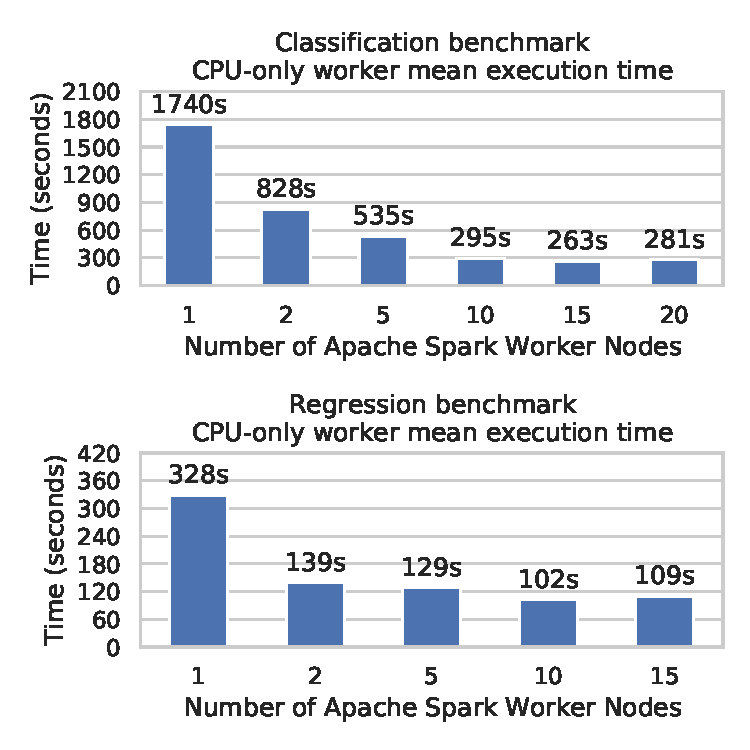
\includegraphics[scale=1]{images/07_evaluation/overall_cpu}
\caption{Basic architecture of a GitLab CI/CD pipeline - Source: Authors own model, based on \cite{Gitlab2020Docs}.}
\label{fig:07_mortgage_static-cpu_results}
\end{figure}
% Explain fig
FIG XY shows the mean execution times for both benchmarks.
% Best results
The classification benchmark achieved the best performance with 15 worker nodes with an overall speed-up of 6.61x in comparison to 1 worker node. The regression benchmark achieved best using 10 worker nodes with an improvement of 3.21x in comparison to 1 worker node.
%  Execution time increase
It can be seen, that for both benchmarks the mean time increased for the last two experiments. For the classification benchmark, the execution time increased by 18 seconds when using 20 worker nodes. Furthermore, the execution time increased by 7 seconds for the regression benchmark when using 15 worker nodes.
% Over provisioning
This performance decrease is caused by over-provisioning the Apache Spark cluster. Too many worker nodes manage the available resources poorly.
% Appendix
The performance data for all iteration of both benchmarks is available at ANHANG A.


% ===========================================
% ===========================================
\section{GPU Acceleration}
% Intro
To explore the impact of GPU accelerated Apache Spark worker nodes, two GPUs of the DGX are available.
%
The benchmarks have been performed with two different cluster configurations. First, both benchmarks were tested with one worker node in the cluster and second with two worker nodes. Each worker node allocates a GPU.
% vs figure
\begin{figure}[h]
\centering
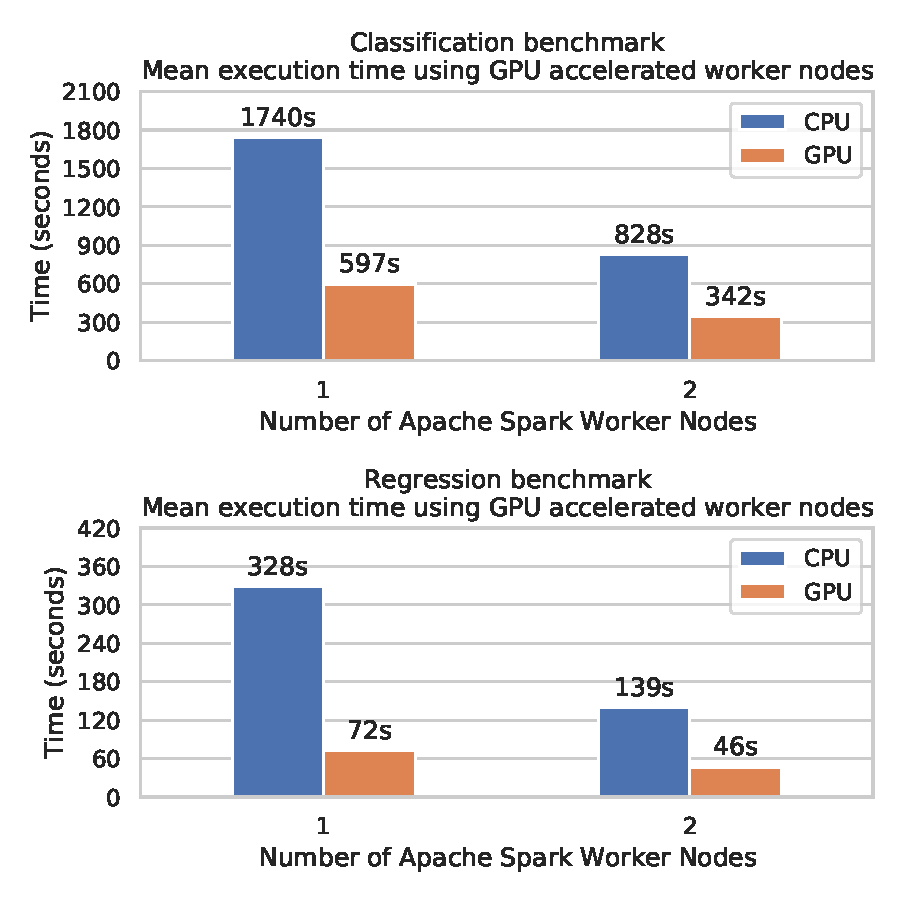
\includegraphics[scale=1]{images/07_evaluation/overall_cpu_vs_gpu}
\caption{Basic architecture of a GitLab CI/CD pipeline - Source: Authors own model, based on \cite{Gitlab2020Docs}.}
\label{fig:07_gpu_results}
\end{figure}
% Explain results
The experiment results are illustrated in FIG XY. 
% vs
The mean execution times using GPU accelerated worker nodes are plotted against the mean execution times using CPU-only worker nodes.
% overall
Overall, GPU accelerated worker nodes significantly outperformed CPU-only worker nodes.
% classification
For the classification algorithm, Apache Spark performed best using two GPUs with an improvement of 2.42x in comparison of two CPU-only worker nodes. Using one GPU accelerated worker node had a speed-up of 2.91x in comparison to one CPU-only worker node.
% regression
The improvement of GPU accelerated worker nodes is noticeable for the regression benchmark as well. Compared to CPU-only worker nodes, using 2 GPUs increases the execution time by 3.02x and 4.55x using 1 GPU.


\paragraph{}
% The table
\Tab{table:07_gpu_overall_results} shows the overall results by comparing the CPU and GPU results.
% GPU outperforms
GPU accelerated worker nodes outperformed their CPU-only equivalent.
% classification
Using 5 CPU-only worker nodes achieved to outperform 1 GPU accelerated worker node by 62s. 10 CPU-only worker were able to outperform 2 GPU accelerated worker nodes by 47s.
% regression
However, CPU-only worker nodes were not able to outperform GPU accelerated worker nodes in the regression benchmark. The best CPU-only result was achieved with 10 worker nodes with 102 seconds. This result is 30s higher than using 1 GPU accelerated worker nodes and 56s higher than 2 GPU accelerated worker nodes.


% Results as table
\begin{table}[]
\centering
\begin{tabular}{@{}l|ll|ll@{}}
\toprule
                  & \multicolumn{2}{c|}{Classification}                & \multicolumn{2}{c}{Regression}                    \\
Number of workers & \multicolumn{1}{c}{CPU} & \multicolumn{1}{c|}{GPU} & \multicolumn{1}{c}{CPU} & \multicolumn{1}{c}{GPU} \\ \midrule
1  & 1740s & 597s & 328s & 72s \\
2  & 828s  & 342s & 139s & 46s \\
5  & 535s  &      & 129s &     \\
10 & 295s  &      & 102s &     \\
15 & 263s  &      & 109s &     \\
20 & 281s  &      &      &     \\ \bottomrule
\end{tabular}
\caption{asfdsfg}
\label{table:07_gpu_overall_results}
\end{table}


% ===========================================
% ===========================================
\section{Auto-Scaler}
% Intro
To test the impact of the Auto-Scaler while training machine learning applications, both benchmarks have been tested with different configurations. \Tab{table:07_auto-scaler_config_parameter} shows the Auto-Scaler configuration parameters for each benchmark.
% Wheres it from
The configuration parameters are choosen in accordance to the results of the static worker experiment.
% Max worker
The classification benchmark achieved best using 15 CPU-only worker nodes and the regression benchmark using 10 CPU-only nodes.
% recurrence
The recurrence factor is set to 1 for both benchmarks. As illustrated in FIG XY, only 2 performance spikes at he beginning and at the end occured. Overall there havent been much oscillation during the training. Having a higher recurrence factor would possibly lead to no scaling action.
% CPU utilization
The CPU utilization values have been chosen in accordance to the minimum and maximum values of the static worker experiment.
% The configurations
\begin{table}[]
\centering
\begin{tabular}{@{}l|ll@{}}
\toprule
Parameter               & Classification & Regression \\ \midrule
Interval                & 5 seconds      & 5 seconds  \\
Recurrence factor       & 1              & 1          \\
Cooldown period         & 60 seconds     & 60 seconds \\
Target CPU utilization  & 5\%           & 5\%        \\
Minimum CPU utilization & 5\%           & 2\%       \\
Maximum CPU utilization & 25\%           & 10\%       \\
Minimum worker nodes    & 2              & 2         \\
Maximum worker nodes    & 15              & 10         \\ \bottomrule
\end{tabular}
\caption{Auto-Scaler configuration parameter}
\label{table:07_auto-scaler_config_parameter}
\end{table}


% Figure
\begin{figure}[h]
\centering
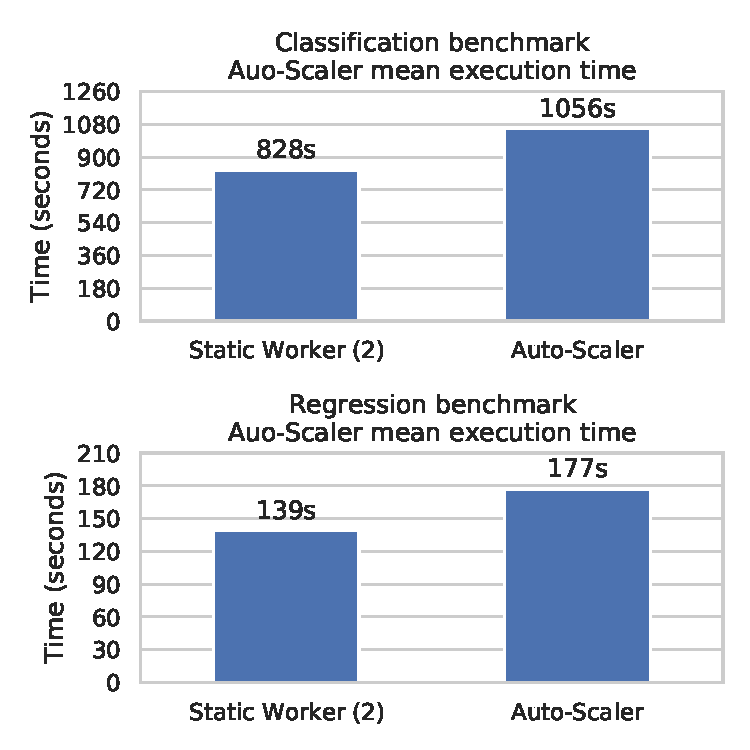
\includegraphics[scale=1]{images/07_evaluation/overall_auto-scaler}
\caption{Basic architecture of a GitLab CI/CD pipeline - Source: Authors own model, based on \cite{Gitlab2020Docs}.}
\label{fig:07_auto-scaler_results}
\end{figure}
% Explain
The results, illustrated in \Fig{fig:07_auto-scaler_results}, showed that scaling the number of Apache Spark worker nodes during the training of a machine learning model increased the execution time of the spark-jobs.
% Classification
In the classification benchmark, the \textit{Auto-Scaler} caused an increase of 228 seconds in comparison of no auto-scaling.
% Regression
Dynamically scaling worker nodes during the regression benchmark increased the mean time by 38 seconds.
% Meaning
The performance decrease of horizontally scaling worker nodes is possible caused that Apache Spark is not able to efficiently distribute the workload during that time. In relation, the increase for the regression benchmark is higher.
